\documentclass[18pt]{beamer}

\IfFileExists{skript.sty}{\usepackage{skript}}{\usepackage{../skript}}

\title[Einfache Wurzeln]{Endliche Spiegelungsgruppen:\\
Einfache Wurzeln}
\author{Pavel Zwerschke}
\date{17. Juni 2019}

\usetheme{Berlin}

\begin{document}

\begin{frame}
    \maketitle
\end{frame}

\begin{frame}
    \tableofcontents
\end{frame}

\section{Wiederholungen Wurzeln}

\begin{frame}{Wurzel}
    Spiegelung an Hyperebene \( \scrP \) 
    lässt sich durch einen Vektor
    \( 0 \neq r \in \scrP^{\bot} \)
    beschreiben:
    \[ s_r(x) = x 
    - 2\frac{\scalarprod{x}{r}}{\scalarprod{r}{r}} r \]
    Es gilt \( \forall x \in \scrP: s_r(x) = x \) 
    und \( s_r(r) = -r \).

    Da Basis \( B \subset \scrP \cup \set{r} \) 
    existiert, folgt aus linearer Fortsetzung, dass 
    \( s_r \) Spiegelung an \( \scrP \) darstellt.

    Außerdem gilt \( s_r^2 = 1 \).

    \( \Rightarrow \pm r \) sind Wurzeln von \( s_r \).

    \( \Delta = \set{ r \;\vert\; r \text{ ist Wurzel} } \) 
    nennen wir Wurzelsystem.
\end{frame}
\section{Positive und einfache Wurzeln}
\begin{frame}{Problem mit Wurzelsystemen}
    Problem: \( \Delta \) kann sehr groß werden.

    Lösungsansatz: Suchen nach linear unabhängigen 
    Untermengen von \( \Delta \), mit denen \( \Delta \)
    konstruiert werden kann.
\end{frame}

\begin{frame}{\( \Delta_t^+ \) und \( \Delta_t^- \)}
    Sei \( t \in V \) so, dass \( \scalarprod{t}{r} \neq 0 
    \; \forall r \in \Delta \).\\
    \( \Delta \) lässt sich in zwei Teilmengen 
    \( \Delta_t^+ = 
    \set{r \in \Delta \;\vert \; \scalarprod{t}{r} > 0} \) 
    und \( \Delta_t^- = 
    \set{r \in \Delta \;\vert \; \scalarprod{t}{r} < 0} \) 
    aufteilen.\\
    % geometrisch gesehen liegen Delta^+ und Delta^- 
    % auf unterschiedlichen Hyperebenen von 
    % t^\bot
    Sei \( r \in \Delta \). \( \Rightarrow -r \in \Delta \), 
    da \( \scalarprod{t}{-r} = -\scalarprod{t}{r} \).\\
    \( \Rightarrow r \) und \( -r \) sind in 
    gegensätzlichen Mengen.
    \[ \Rightarrow \abs{\Delta_t^+} = \abs{\Delta_t^-}. \]
\end{frame}

\section{Einfache Wurzelsysteme}
\begin{frame}{Definition \( t \)-Basis}
    \( \Pi \subset \Delta_t^+ \) heißt \( t \)-Basis, 
    wenn gilt:
    \begin{itemize}
        \item Jedes \( r \in \Delta_t^+ \) ist 
        eine Linearkombination mit ausschließlich 
        nichtnegativen Koeffizienten.
        \item \( \Pi \) ist minimal.
    \end{itemize}
    Es existiert mindestens eine \( t \)-Basis, 
    da \( \Delta \) endlich ist.\\
    Da \( \Delta_t^+ = - \Delta_t^- \), ist jedes 
    \( r \in \Delta_t^- \) eine Linearkombination 
    mit ausschließlich nichtpositiven Koeffizienten.\\
    \( \Pi \) ist eine Basis. % TODO zu beweisen?
\end{frame}

\begin{frame}{Definition \(t\)-positiv}
    \( x \in V \) heißt \(t\)-positiv, wenn 
    die Linearkombination von \(x\) zur 
    Basis ausschließlich nichtnegativ ist.\\
    Analog für \( t \)-negativ.\\
    Hängt nicht von \( \Pi \) ab, da \( \Pi \) 
    eindeutig.%todo beweisen?
\end{frame}

\begin{frame}{Orthogonalität} % todo besserer Titel
    \begin{satz} % Proposition 4.1.4
        % satz 1
        Seien \( r_i, r_j \in \Pi, i \neq j \) und 
        \( \lambda_i, \lambda_j \in \R_+ \). 
        Der Vektor \( x = \lambda_i r_i - \lambda_j r_j \) 
        ist weder \( t \)-positiv noch \( t \)-negativ.
    \end{satz}
\end{frame}

\begin{frame}
    \begin{bew}
        Wenn \(x\) positiv wäre, könnten 
        wir schreiben 
        \[ x = \lambda_i r_i - \lambda_j r_j 
        = \sum_{k=1}^m \mu_k r_k \]
        mit allen \( \mu_i \geq 0 \).
        Fall 1 \( \lambda_i \leq \mu_i \):
        \[ \Leftrightarrow 0 
        = - \lambda_i r_i + \lambda_j r_j 
        + \sum_{k=1}^m \mu_k r_k \]
        
        \renewcommand{\qedsymbol}{}
    \end{bew}
\end{frame}

\begin{frame}
    \begin{bew}
        \[ \Leftrightarrow 0 = (\mu_i - \lambda_i)
        r_i + (\mu_j + \lambda_j) 
        r_j + 
        \sum_{
            \substack{k \in \set{1,\ldots, m}\\k \neq i,j}}
        \mu_k r_k \]
        Dauraus folgt 
        \[ 0 = \scalarprod{t}{ 
            (\mu_i - \lambda_i) r_i + (\mu_j + \lambda_j) r_j 
        + \sum_{\substack{k \in \set{1,\ldots, m}\\k \neq i,j}}
        \mu_k r_k
        } \geq \lambda_j \scalarprod{t}{r_j} > 0. 
        \text{ \Lightning} \]

        \renewcommand{\qedsymbol}{}
    \end{bew}
\end{frame}

\begin{frame}
    \begin{bew}
        Wenn \( \lambda_i > \mu_i \), dann gilt 
        \[ (\lambda_i - \mu_i) r_i
        = (\mu_j + \lambda_j) r_j 
        + \sum_{\substack{k \in \set{1,\ldots, m}\\k \neq i,j}}
        \mu_k r_k. \]
        Dann ließe sich \( r_i \) als eine 
        nichtnegative Linearkombination von 
        \( \Pi \setminus \set{r_i} \) darstellen. 
        \Lightning{} zur Minimalität von 
        \( \Pi \).

        Wenn \( x \) negativ ist, müsste \( -x \) 
        positiv sein, was nicht möglich ist.
    \end{bew}
\end{frame}

\begin{frame}{Spiegelung einer Wurzel}
    % satz 2
    \begin{satz} % Proposition 1.4.5
        Seien \( r_i, r_j \in \Pi, i \neq j \), es 
        sei \( S_i \) die Spiegelung an \( r_i \). 

        Dann ist \( S_i r_i \in \Delta_t^+ \) und 
        \( \scalarprod{r_i}{r_j} \leq 0 \).
    \end{satz}

    \begin{bew}
        Da \( S_i r_j \in \Delta \), ist \( S_i r_j \) 
        entweder positiv oder negativ. Da 
        \[ S_i r_j = r_j - 2 \scalarprod{r_j}{r_i} r_i, \]
        mit \( \lambda_j = 1 \), muss 
        \( \lambda_i \geq 0 \), da sonst 
        \( S_i r_i \notin \Delta \). 

        \( \Rightarrow \scalarprod{r_i}{r_j} \leq 0 
        \Rightarrow S_i r_j \) 
        positiv.
    \end{bew}
    % geometrische Bedeutung:
    % <r_i, r_j> \leq 0 bedeutet, dass Winkel zwischen 
    % r_i und r_j stumpf ist, da skalarprod der cosinus vom winkel 
    % ist.
\end{frame}

\begin{frame}
    % satz 3
    \begin{satz} % Proposition 1.4.6
        Seien \( x_1, \ldots, x_m \in V \) alle auf derselben 
        Seite einer Hyperebene \( \scrP \). \\
        Falls \( \scalarprod{x_i}{x_j} \leq 0 \) immer wenn 
        \( i \neq j \), dann ist \( \set{x_1, \ldots, x_m} \) 
        linear unabhängig.
    \end{satz}

    \begin{bew}
        Wenn das der Fall wäre, dann gäbe es 
        \( \lambda_i, \mu_i \geq 0 \) mit 
        manchen \( \lambda_i > 0 \), sodass 
        \[ \sum_{i=1}^k \lambda_i x_i 
        = \sum_{i=k+1}^m \mu_i x_i. \]

        \renewcommand{\qedsymbol}{}
    \end{bew}
\end{frame}

\begin{frame}
    \begin{bew}
        Dann gilt 
        \begin{align*}
            0 \leq \norm{\sum_{i=1}^k \lambda_i x_i}^2 
            &= \scalarprod{\sum_{i=1}^{k} \lambda_{i} x_{i}}{
            \sum_{j=1}^{k} \lambda_{j} x_{j}} \\
            &= \scalarprod{\sum_{i=1}^{k} \lambda_{i} x_{i}}{
            \sum_{j=k+1}^{m} \mu_{j} x_{j}} \\
            &= \sum_{i=1}^{k} \sum_{j=k+1}^{m} \lambda_{i} \mu_{j}
            \scalarprod{x_i}{x_j} 
            \leq 0. % nach Voraussetzung
        \end{align*}
        
        \renewcommand{\qedsymbol}{}
    \end{bew}
\end{frame}
\begin{frame}
    \begin{bew}
        Es gilt jedoch nun 
        \[ 0 = \scalarprod{\sum_{i=1}^{k} \lambda_i x_i}{x} 
        = \sum_{i=1}^k \lambda_i \scalarprod{x_i}{x} > 0. \text{ \Lightning{}} \]
        % da manche lambda_i > 0
        Deshalb muss \( \set{x_1, \ldots, x_m} \) linear 
        unabhängig sein.
    \end{bew}
\end{frame}

\begin{frame}
    % Theorem 4
    \begin{theorem} % Theorem 1.4.8
        Sei \( \Pi \) eine \(t\)-Basis von \( \Delta \). Dann ist 
        \( \Pi \) eine Basis für \( V \).
    \end{theorem}

    \begin{bew}
        \begin{itemize}
            \item \( \Delta \) erzeugt \( V \). (s. Vortrag \gqq{Wurzelsysteme})\\
            Da jedes \( r \in \Delta \) eine Linearkombination von \( \Pi \) ist, 
            ist \( \Pi \) Erzeugendensystem.
            \item \( \Delta \) ist nach Satz 2 und 3 linear unabhängig.
        \end{itemize}
        \( \Rightarrow \Pi \) ist eine Basis von \(V\).
    \end{bew}
\end{frame}

\begin{frame}
    % Satz 5
    \begin{satz} % Proposition 4.1.8
        Es gibt nur eine \( t \)-Basis von \( \Delta \).
    \end{satz}
    % TODO beweis nötig?
\end{frame}

\section{Beispiele}
\begin{frame}{Beispiele}
    Sei \( \mathscr{G} = \mathscr{H}_2^4 \), 
    die vier Spiegelungen in \( \mathscr{G} \) 
    generieren es.
    \[ \Delta = \set{ \pm(1,0), \pm(0,1), (\pm 1, \pm 1) }. \]
    Wähle \( t = 2( \cos(\frac{3\pi}{8}), \sin(\frac{3\pi}{8}) ) \).

    \begin{columns}[c]
        \begin{column}{0.7\textwidth}
            \begin{align*}
                \Rightarrow \Delta_+ 
                &= \set{(1,0), (1,1), (0,1), (-1,1)}, \\
                \Pi &= \set{ (1,0), (-1,1) }.
            \end{align*}
        \end{column}
        \begin{column}{0.3\textwidth}
         \begin{figure}
            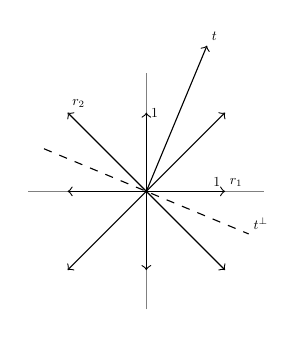
\begin{tikzpicture}
                \draw[thin, gray] (-1.5,0) -- (1.5,0);
                \draw[thin, gray] (0,-1.5) -- (0,1.5);
                \draw[->] (0,0) -- (0,1) node[right, scale=0.5] {\( 1 \)};
                \draw[->] (0,0) -- (0,-1);
                \draw[->] (0,0) -- (-1,0);
                \draw[->] (0,0) -- (1,0) node[above right, scale=0.5] {\( r_1 \)}
                node[above left, scale=0.5] {\( 1 \)};
                \draw[->] (0,0) -- (-1, 1) node[above right, scale=0.5] {\( r_2 \)};
                \draw[->] (0,0) -- (-1,-1);
                \draw[->] (0,0) -- (1,1);
                \draw[->] (0,0) -- (1,-1);
                \draw[->] (0,0) -- (0.77, 1.85) node[above right, scale=0.5] {\( t \)};
                \draw[dashed] (-1.3,-0.77 / 1.85 * -1.3) -- (1.3, -0.77 / 1.85 * 1.3) 
                node[above right, scale=0.5] {\( t^\bot \)};
            \end{tikzpicture}
          \end{figure}
        \end{column}
      \end{columns}
\end{frame}

\section{Weitere Sätze}
\begin{frame}
    \begin{satz}
        Sei \( S_i \) die Spiegelung an 
        \( r_i \in \Pi = \set{r_1, \ldots, r_n} \).
        Wenn \( r \in \Delta^+ \) und \( r_i \neq r \), 
        dann gilt \( S_i r \in \Delta^+ \).
    \end{satz}
\end{frame}

% todo

\end{document}